\documentclass[aspectratio=169]{beamer}
% SGSSS Beamer Preamble — shared across all lectures
% Brand colours from SGSSS logo

\usetheme{metropolis}

% --- Colour definitions ---
\definecolor{sgsssMagenta}{HTML}{A3217A}
\definecolor{sgsssGreen}{HTML}{2D6A3F}
\definecolor{sgsssBlack}{HTML}{1D1D1B}
\definecolor{sgsssWhite}{HTML}{FFFFFF}
\definecolor{sgsssLightGrey}{HTML}{F5F5F5}

% --- Metropolis colour overrides ---
\setbeamercolor{palette primary}{bg=sgsssMagenta, fg=sgsssWhite}
\setbeamercolor{title separator}{fg=sgsssGreen}
\setbeamercolor{progress bar}{fg=sgsssGreen, bg=sgsssLightGrey}
\setbeamercolor{frametitle}{bg=sgsssMagenta, fg=sgsssWhite}
\setbeamercolor{alerted text}{fg=sgsssMagenta}
\setbeamercolor{example text}{fg=sgsssGreen}
\setbeamercolor{block title}{bg=sgsssMagenta, fg=sgsssWhite}
\setbeamercolor{block body}{bg=sgsssLightGrey, fg=sgsssBlack}
\setbeamercolor{block title example}{bg=sgsssGreen, fg=sgsssWhite}
\setbeamercolor{block body example}{bg=sgsssLightGrey, fg=sgsssBlack}
\setbeamercolor{normal text}{fg=sgsssBlack}

% --- Fonts ---
\usepackage[T1]{fontenc}
\usepackage[sfdefault]{FiraSans}
\usepackage{FiraMono}
\setbeamerfont{frametitle}{size=\large}

% --- Packages ---
\usepackage{graphicx}
\usepackage{hyperref}
\usepackage{array}
\usepackage{booktabs}
\usepackage{minted}
\usepackage{fontawesome5}

% --- TikZ ---
\usepackage{tikz}
\usetikzlibrary{arrows.meta, positioning, shapes.geometric, trees, calc, decorations.pathmorphing, decorations.pathreplacing, fit, backgrounds}

% Reusable TikZ styles
\tikzset{
    server node/.style={rectangle, draw=sgsssGreen, fill=sgsssGreen!10, thick, minimum width=2.5cm, minimum height=1.2cm, align=center, font=\small},
    client node/.style={rectangle, draw=sgsssMagenta, fill=sgsssMagenta!10, thick, minimum width=2.5cm, minimum height=1.2cm, align=center, font=\small},
    api node/.style={rectangle, draw=sgsssGreen, fill=sgsssGreen!15, thick, rounded corners, minimum width=2.5cm, minimum height=1.2cm, align=center, font=\small},
    data node/.style={rectangle, draw=sgsssBlack, fill=sgsssLightGrey, thick, minimum width=2cm, minimum height=1cm, align=center, font=\small},
    arrow style/.style={-{Stealth[length=3mm]}, thick, sgsssBlack},
    html tag/.style={rectangle, draw=sgsssMagenta, fill=sgsssMagenta!8, rounded corners=2pt, font=\ttfamily\small, inner sep=4pt},
    json key/.style={rectangle, draw=sgsssGreen, fill=sgsssGreen!8, rounded corners=2pt, font=\ttfamily\small, inner sep=4pt},
}

% --- Minted configuration ---
\setminted{
    fontsize=\footnotesize,
    frame=leftline,
    framesep=2mm,
    baselinestretch=1.1,
    bgcolor=sgsssLightGrey,
    breaklines,
    linenos=false,
}
\setminted[python]{style=friendly}
\setminted[r]{style=friendly}

% --- Convenience commands ---
\newcommand{\pythoncode}[1]{\mintinline{python}{#1}}
\newcommand{\rcode}[1]{\mintinline{r}{#1}}
\newcommand{\httpstatus}[2]{\texttt{#1} \textit{#2}}

% --- Footer (page numbers only; logo on title slide only) ---
\setbeamertemplate{frame footer}{%
    \insertframenumber/\inserttotalframenumber%
}

% --- Metadata ---
\author{Dr Diarmuid McDonnell}
\institute{Braw Data Ltd \and Gradel Institute of Charity, University of Oxford}
\date{24 February 2026}


\title{Collecting Digital Data:\\The Role of Web-scraping and APIs}
\subtitle{SGSSS Training Course}

\begin{document}

% -------------------------------------------------------
% Slide 1: Title
% -------------------------------------------------------
{
\setbeamertemplate{frame footer}{}
\begin{frame}[plain]
    \begin{center}
        \includegraphics[height=2.5cm]{../img/SGSSS_Stacked.png}\\[0.8cm]
        {\Large\bfseries\color{sgsssMagenta} Collecting Digital Data}\\[0.2cm]
        {\large The Role of Web-scraping and APIs}\\[0.6cm]
        {\normalsize Dr Diarmuid McDonnell}\\[0.1cm]
        {\small Braw Data Ltd \(\cdot\) Gradel Institute of Charity, University of Oxford}\\[0.3cm]
        {\small 24 February 2026}
    \end{center}
\end{frame}
}

% -------------------------------------------------------
% Slide 2: About the instructor
% -------------------------------------------------------
\begin{frame}{About the Instructor}
    \textbf{Dr Diarmuid McDonnell}
    \begin{itemize}
        \item Director, \textbf{Braw Data Ltd}
        \item Visiting Fellow, \textbf{Gradel Institute of Charity}, University of Oxford
        \item Research: geographic distribution of civil society activity
        \item Background in quantitative social science and data science
    \end{itemize}
    \vspace{0.3cm}
    {\small \faIcon{globe} \url{https://www.brawdata.co.uk}}\\
    {\small \faIcon{university} \url{https://www.gradelinstituteofcharity.co.uk/diarmuid-mcdonnell}}
\end{frame}

% -------------------------------------------------------
% Slide 3: Course outline
% -------------------------------------------------------
\begin{frame}{Course Outline}
    \footnotesize
    \begin{tabular}{@{}lll@{}}
        \toprule
        \textbf{Time} & \textbf{Session} & \textbf{Format} \\
        \midrule
        10:00--10:30 & Welcome \& How the Web Works & Lecture \\
        10:30--11:15 & \alert{Practical 1: Web Scraping} & Colab notebook \\
        11:15--11:30 & Break & \\
        11:30--11:45 & What Are APIs? & Lecture \\
        11:45--12:45 & \alert{Practical 2: UK Police API} & Colab notebook \\
        12:45--13:30 & Lunch & \\
        13:30--13:45 & API Landscape Survey & Lecture \\
        13:45--14:45 & \alert{Practical 3: API Challenge} & Colab notebook \\
        14:45--15:00 & Break & \\
        15:00--15:15 & LLMs as Coding Assistants & Lecture \\
        15:15--15:50 & \alert{Practical 4: LLM Showdown} & Colab notebook \\
        15:50--16:00 & Wrap-up \& Q\&A & \\
        \bottomrule
    \end{tabular}
\end{frame}

% -------------------------------------------------------
% Slide 4: Getting set up
% -------------------------------------------------------
\begin{frame}{Getting Set Up}
    \begin{block}{What you need}
        \begin{itemize}
            \item A \textbf{Google account} (for Google Colab)
            \item A web browser (Chrome recommended)
        \end{itemize}
    \end{block}

    \begin{block}{How to access the notebooks}
        \begin{enumerate}
            \item Go to the course \textbf{README} (link shared on Teams/email)
            \item Click the \textbf{Open in Colab} badge for your chosen language
            \item Sign in with your Google account
            \item You're ready to go!
        \end{enumerate}
    \end{block}

    \vspace{0.2cm}
    {\small \faIcon{info-circle} No software installation required --- everything runs in the browser.}
\end{frame}

% -------------------------------------------------------
% Slide 5: Why collect digital data?
% -------------------------------------------------------
\begin{frame}{Why Collect Digital Data?}
    \begin{itemize}
        \item \textbf{Government open data} --- policy evaluation, freedom of information, public spending
        \item \textbf{Social media} --- opinion analysis, political discourse, misinformation
        \item \textbf{Organisational websites} --- third-sector research, corporate governance, labour markets
        \item \textbf{Administrative records} --- health, education, justice system data via APIs
    \end{itemize}

    \vspace{0.5cm}
    \begin{alertblock}{Key idea}
        The web is a vast, continuously updated source of social science data --- but accessing it requires the right tools and techniques.
    \end{alertblock}
\end{frame}

% -------------------------------------------------------
% Slide 6: How the web works
% -------------------------------------------------------
\begin{frame}{How the Web Works}
    \begin{center}
    
\begin{tikzpicture}[node distance=5cm]
        % Nodes
        \node[client node] (client) {\faIcon{laptop}\\Your Computer};
        \node[server node, right=of client] (server) {\faIcon{server}\\Web Server};

        % Arrows — spread vertically to avoid overlap
        \draw[arrow style] ([yshift=0.5cm]client.east) -- ([yshift=0.5cm]server.west)
            node[midway, above, font=\small] {HTTP Request}
            node[midway, below, font=\footnotesize\ttfamily, text=sgsssMagenta] {GET https://example.com};
        \draw[arrow style] ([yshift=-0.5cm]server.west) -- ([yshift=-0.5cm]client.east)
            node[midway, below, font=\small] {HTTP Response}
            node[midway, above, font=\footnotesize\ttfamily, text=sgsssGreen] {200 OK + HTML/JSON};
    \end{tikzpicture}
    \end{center}

    \vspace{0.2cm}
    \small
    \textbf{Common HTTP status codes:}\\[0.15cm]
    \footnotesize
    \httpstatus{200}{OK} \(\cdot\)
    \httpstatus{301}{Moved Permanently} \(\cdot\)
    \httpstatus{302}{Found (Redirect)} \(\cdot\)
    \httpstatus{400}{Bad Request} \(\cdot\)
    \httpstatus{401}{Unauthorised} \(\cdot\)
    \httpstatus{403}{Forbidden} \(\cdot\)
    \httpstatus{404}{Not Found} \(\cdot\)
    \httpstatus{429}{Too Many Requests} \(\cdot\)
    \httpstatus{500}{Server Error}
\end{frame}

% -------------------------------------------------------
% Slide 7: HTML basics
% -------------------------------------------------------
\begin{frame}[fragile]{HTML Basics}
    \begin{columns}[T]
        \begin{column}{0.45\textwidth}
            \textbf{HTML tree structure}\\[0.3cm]
            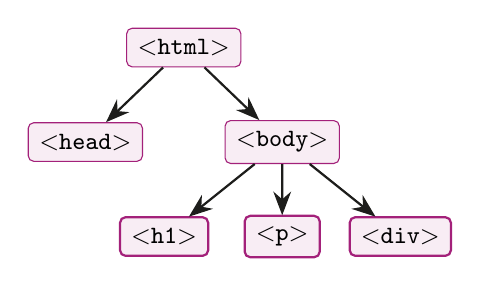
\begin{tikzpicture}[
                level distance=1.2cm,
                level 1/.style={sibling distance=2.5cm},
                level 2/.style={sibling distance=1.5cm},
                edge from parent/.style={draw, arrow style},
                every node/.style={html tag}
            ]
                \node {\textless html\textgreater}
                    child { node {\textless head\textgreater} }
                    child { node {\textless body\textgreater}
                        child { node {\textless h1\textgreater} }
                        child { node {\textless p\textgreater} }
                        child { node {\textless div\textgreater} }
                    };
            \end{tikzpicture}\\[0.2cm]
            {\small Tags define structure and meaning}
        \end{column}
        \begin{column}{0.5\textwidth}
            \textbf{Example HTML}
            \begin{minted}[fontsize=\scriptsize]{html}
<html>
  <head>
    <title>My Page</title>
  </head>
  <body>
    <h1>Welcome</h1>
    <p>Hello, world!</p>
  </body>
</html>
\end{minted}
        \end{column}
    \end{columns}
\end{frame}

% -------------------------------------------------------
% Slide 8: Structured vs unstructured data
% -------------------------------------------------------
\begin{frame}[fragile]{Structured vs Unstructured Data}
    \begin{columns}[T]
        \begin{column}{0.47\textwidth}
            \textbf{Unstructured (HTML)}
            \begin{minted}[fontsize=\scriptsize]{html}
<div class="person">
  <h2>Jane Smith</h2>
  <p>Age: 34</p>
  <p>City: Edinburgh</p>
</div>
\end{minted}
            \begin{itemize}
                \small
                \item Designed for \textbf{human} reading
                \item Structure can change without notice
                \item Requires parsing to extract data
            \end{itemize}
        \end{column}
        \begin{column}{0.47\textwidth}
            \textbf{Structured (JSON)}
            \begin{minted}[fontsize=\scriptsize]{json}
{
  "name": "Jane Smith",
  "age": 34,
  "city": "Edinburgh"
}
\end{minted}
            \begin{itemize}
                \small
                \item Designed for \textbf{machine} reading
                \item Consistent, documented format
                \item Easy to convert to tables
            \end{itemize}
        \end{column}
    \end{columns}
\end{frame}

% -------------------------------------------------------
% Slide 9: Ethics and legality
% -------------------------------------------------------
\begin{frame}{Ethics and Legality}
    \begin{itemize}
        \item \faIcon{robot} \textbf{Check robots.txt} --- websites specify what can be crawled
        \item \faIcon{file-contract} \textbf{Read Terms of Service} --- some sites explicitly prohibit scraping
        \item \faIcon{clock} \textbf{Respect rate limits} --- don't overwhelm servers with requests
        \item \faIcon{user-shield} \textbf{Consider personal data} --- GDPR applies to identifiable information
        \item \faIcon{plug} \textbf{Prefer APIs when available} --- structured, legal, reliable
        \item \faIcon{spider} \textbf{Web scraping as last resort} --- use only when no API exists
    \end{itemize}

    \vspace{0.4cm}
    \begin{exampleblock}{Note}
        We will discuss ethical and legal considerations throughout the day as they arise in each practical.
    \end{exampleblock}
\end{frame}

% -------------------------------------------------------
% Slide 10: Next up
% -------------------------------------------------------
\begin{frame}{Next Up}
    \begin{center}
        {\Large \alert{Practical 1: Web Scraping}}\\[0.5cm]
        \begin{itemize}
            \item Extract text from a simple web page
            \item Scrape data across multiple pages
            \item Save structured data to a file
        \end{itemize}
        \vspace{0.5cm}
        {\normalsize Open the \textbf{Practical 1} notebook in Google Colab\\(Python or R --- your choice!)}
    \end{center}
\end{frame}

\end{document}
